% -----------------------------------------------------------------------------
% Metodologia
% -----------------------------------------------------------------------------

\chapter{Metodologia}
\label{chap:metodologia}
\section{Disponibilidade dos recursos deste trabalho}

Todos os componentes definidos nesse trabalho estão em um repositório público no  Github: \href{https://github.com/felipefrocha/esufmg-tcc}{https://github.com/felipefrocha/esufmg-tcc}, garantindo a livre apreciação da comunidade não só científica, mas a todos os interessados na contribuição ou utilização sob a licença pública geral GNU versão 3 \cite{foss2022}.

\section{Especificação dos nós integrantes do  \emph{cluster} de baixo custo}

A formação do  \emph{cluster} é de máquinas físicas que possuem custo e capacidade computacionais mais baixos, com configurações comumente encontradas em computadores do tipo \emph{desktops}, como os utilizados em residências, escritórios e laboratórios de informática genéricos.

A primeira versão dessa solução foi realizada de maneira simulada, utilizando ambiente virtualizado com VMs que foram provisionadas em \emph{hypervisors} do tipo 2 \cite{comer_cloud_2021} (\emph{hosted} \emph{hypervisor}), para garantir a simplicidade da implementação dos conceitos abordados no trabalho e validar a abordagem de provisionamento, configuração e \emph{deploy} de aplicações testes e laboratório das ferramentas de monitoramento que são utilizadas, a serem descritas na sessão \ref{chap:monitor}.

O desenvolvimento desse trabalho é o provisionamento do  \emph{cluster} nos ambientes de teste configurados como descrito na sessão \ref{sec:abordagem}, sendo que algumas premissas são utilizadas, como o uso de mesmo sistema operacional e versão em cada um desses computadores, garantindo a redução de configuração necessária para a implementação. Outra premissa utilizada para esse estudo é a utilização de uma rede comum aos computadores.

O aproveitamento de computadores comuns já existentes e subutilizados, seja por uso abaixo de sua capacidade ou ainda intervalos de ociosidade, qualifica o baixo custo da formação do  \emph{cluster} em questão, apresentando CAPEX (capital expenditure),  ou investimento inicial mínimo, se não zero.
\section{Plataforma de orquestração de carga de trabalho}

A plataforma de  \emph{cluster} e orquestração de cargas de trabalho utilizadas nesse trabalho é o Kubernetes. A arquitetura de implementação do  \emph{cluster} é de \emph{multi-master} com etcd \cite{etcd2022} (controlador de logs, e estado do  \emph{cluster}) anexado \cite{kubernetes2022}, ou rodando nos mesmos computadores masters do  \emph{cluster}.
A arquitetura apresentada garante  (Figura \ref{fig:kubeadmha}) alta disponibilidade do  \emph{cluster}, importante para que não haja interrupções inesperadas durante a orquestração das cargas de trabalho (execução, disponibilidade e garantia de estado desejado). Ela apenas não garante uma recuperação rápida de quedas dos servidores dos nós (computador/servidor integrante do \emph{cluster}) mestres, significando a perda de todos os estados e, com isso, havendo a necessidade de reconfiguração do  \emph{cluster}. Porém, considerando os recursos limitados, na justificativa desse projeto, a alta disponibilidade de estado, significaria na obrigatoriedade do mesmo número de computadores disponibilizados para etcd e masters para controle dos estados.


\begin{figure}[!ht]
    \centering
    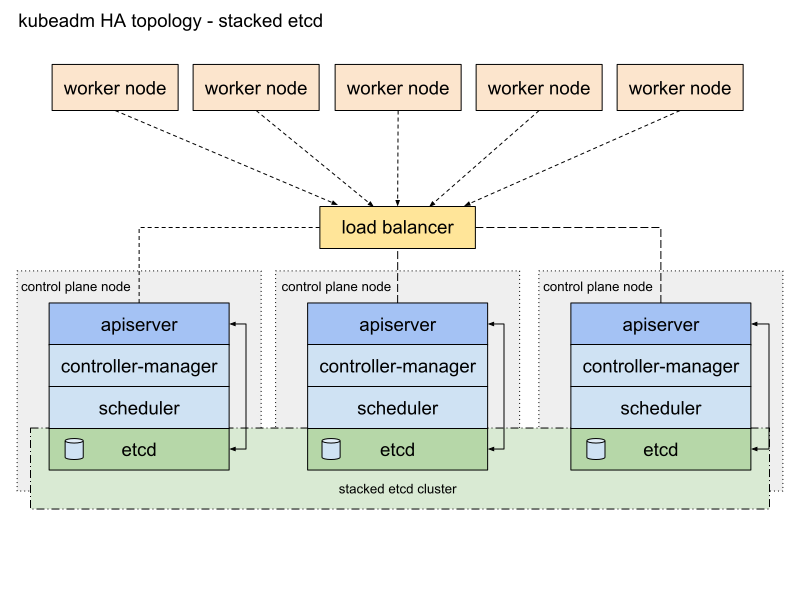
\includegraphics[width=0.8\textwidth]{04-figuras/kubeadm-ha-topology-stacked-etcd.png}
    \caption[Kubernetes Arquitetura de alta disponibilidade]{Kubernetes Arquitetura de alta disponibilidade (Fonte: The Linux Foundation\textregistered, 2021)}
    \label{fig:kubeadmha}
\end{figure}


Toda a implementação da solução e os componentes relacionados estão conteinerizados, possibilitando  sua orquestração pelo  \emph{cluster} de Kubernetes\textregistered. Apenas as configurações dos  \emph{clusters} e seu provisionamento não são conteinerizados. Esses estão disponibilizados em outro repositório específico.
Para ciclo de vida da aplicação e configurações gerais da solução é utilizada uma estratégia de organização de código em monorepo, sendo essa estratégia a utilização de um repositório único para acompanhamento e desenvolvimento de todos os componentes de software e configurações. Isso facilita a visualização, centralização, sincronização e padronização como benefícios primários, conforme citado na literatura, reforçando a adoção dessa estratégia \cite{brito_monorepos_2018}.


\section{Configuração e provisionamento do  \emph{cluster}}

Oito computadores foram utilizados na estruturação do cluster, somando 42 CPUs e 88 GB RAM. Neles foi, inicialmente, instalada a versão LTS (\emph{long term support}) da distribuição de Linux\textregistered \ Ubuntu\textregistered \ \emph{Server} {20.04.3}. Para facilidade de configuração, mantendo a segurança dos \emph{clusters}, todos foram configurados com chaves SSH para acesso remoto. O laboratório Winet do DCC UFMG, parceiro na realização desse trabalho, cedeu uma de suas sub-redes de comprimento /25 (CIDR, \emph{Classless Inter-Domain Routing}).

Para provisionamento do \emph{cluster} é utilizado Ansible\textregistered, da empresa RedHat\textregistered \ que é  um sistema de gerenciamento de configuração (CMS). Sua adoção se deu pela característica minimalista de configuração inicial, facilidade de uso e uma característica fundamental que diminui o \emph{overhead} de operação necessária para sua utilização: não possuir agente instalado no inventário de máquinas gerenciadas.

O principal ganho na utilização de CMS é a manutenção e replicabilidade de uma determinada configuração e, no caso do Ansible, não há necessidade de configuração prévia ou instalação de nenhum binário específico para sua utilização, reduzindo assim a complexidade de sua adoção.

A configuração inicial é realizada pela disponibilidade de: acesso via rede e python instalado na máquina. O gerenciamento dessa  configuração é feita por ativo (asset, ou recurso) relacionado em uma lista de recursos agrupadas, chamada inventário. Também é possível utilizar alguns tipos de autenticação (kerberos, WinRM, SSH etc). O tipo utilizado no trabalho foi o protocolo SSH \cite{noauthor_rfc4254_nodate} por chaves assimétricas, o que garante um nível aceitável de segurança, especialmente quando é possível escolher os algoritmos de criptografia e suas possíveis variações como RSA e ED25519.

\subsection{Orquestração do processamento de ingestão dos dados}

Para obtenção e trabalho com os dados propostos, escolheu-se trabalhar com um fluxo conhecido de mercado, aplicado tanto em rotinas de batelada (\emph{batch}), como em processos de contínuos \emph{stream}. A extração, transformação e carga (ETL) dos dados foi obtida de uma fonte de armazenamento remota por requisição \emph{download}, via endereço de URL (\emph{Uniform Resource Locators}), seguido da transformação (filtragem, sumarização) e carregado em um banco de dados relacional localizado no \emph{cluster}, no caso PostgreSQL\textregistered.

A orquestração das \emph{tasks} (tarefas), no conceito apresentado pela ferramenta {Apache Airflow}\textregistered \ \cite{airflowconcepts}, permite realizar a execução em uma ordem especifica, essa estrutura é definida em uma DAG(\emph{direct aciclic graph}). Em execuções simultâneas e paralelas de tarefas, utilizou-se o modo de execução associado a API (\emph{application programming interface}) do Kubernetes\textregistered. Dessa forma, cada \emph{task} é criada em um novo \emph{pod} com recursos definidos em sua especificação \emph{task} durante o paralelismo dinâmico dos processos(\emph{fanout pattern}).

Essa técnica é comumente associada a padrões de execução \emph{serveless}, usualmente utilizando um processo de subscrição por mensagem dos novos processos. No caso do mapeamento dinâmico das tarefas orquestradas pelo Airflow, uma vez que são utilizados pods independentes por tarefa, podemos estrapolar o termo. Para melhor entendimento pode-se fazer uma comparação com \emph{fork} de processos em processamento paralelo, salvo que no contexto do cluster, o pod (unidade onde a tarefa é executada) pode ou não ser instanciado no mesmo computador de origem do executor, e por meio de \emph{callback} com o \emph{scheduler} do \emph{cluster}  - uma comunicação por um banco de metadados -, o executor gera os pods de execução das tarefas, controla o estado da tarefa e seu retorno.


\section{Monitoramento}
\label{chap:monitor}

São utilizados para monitoramento de execução das cargas de trabalho o Prometheus\textregistered \  e para visualização dos dados Grafana\textregistered, ambos sendo configurados a partir do provisionamento do  \emph{cluster}, ainda com a ferramenta proposta inicialmente Ansible\textregistered. Dessa forma, é possível avaliar parâmetros de taxa de lotação das máquinas base, pelo parâmetro de processador e memória, operações de leitura e escrita no disco e também tráfego de rede. Por meio dessas ferramentas é possível, ainda, avaliar dados de tempo de execução de cargas de trabalho em ambos os ambientes propostos e, assim, poder compará-los quanto a eficiência de uso de hardware.

O tipo de teste de aplicação é um macrobenchmark (system level benchmark) \cite{huge2008,scheepers2014virtualization} comparando parâmetros de uso de CPU, memória e tempo de execução da carga de trabalho proposta na sessão \ref{chap:monitor} deste trabalho. Os parâmetros são avaliados tanto na máquina de suporte ao container, como também os containers em si, bem como o tempo de provisionamento do  \emph{container} da carga de trabalho, tempo de execução e quantidades de falhas.

Esse método USE (Usage, Saturation and Errors) \cite{greg2022} é utilizado para extrair e apresentar métricas e avaliar possíveis problemas. Destaca-se que esse não é o foco do trabalho, mas captura de forma adequada os parâmetros de \emph{hardware} citados acima.

O controle de tempo é através de ferramentas de orquestração {Apache Airflow}\textregistered. O que permite visualizar detalhadamente o tempo de execução, inicio e finalização das tarefas.

\section{Análise de dados}

O banco de dados “Vendas de Medicamentos Controlados e Antimicrobianos - Medicamentos Industrializados”, disponibilizado pelo governo brasileiro (via portal dados.gov.br), é utilizado nesse trabalho. Os anos correspondentes dos dados são no período entre 2014 e 2020 e o banco possui mais de 70 GB  e mais de 530 milhões de linhas sendo, portanto, suficiente para ser utilizado como carga de trabalho.

Um banco de dados contendo todas as prescrições de azitromicina dispensadas por farmácias privadas
e drogarias brasileiras, no período de 2014 a 2020, é construído a partir dos dados processados dos
bancos de “Vendas de Medicamentos Controlados e Antimicrobianos - Medicamentos Industrializados”.
A azitromicina foi escolhida como objeto de análise de consumo para os períodos pré e durante a
pandemia da COVID-19, por se tratar do antimicrobiano – sujeito à venda controlada no Brasil – mas
amplamente indicado para a prevenção ou tratamento da COVID-19, mesmo sem comprovação de
eficácia \cite{santos2021kit}.

As seguintes variáveis são coletadas: apresentação, quantidade dispensada e unidade federativa (UF)
de comercialização de cada medicamento; idade e sexo do paciente.
São mensuradas as tendências de consumo por meio do número unidades dispensadas – caixas ou
frascos –, avaliadas usando o índice de correlação tau de Kendall para a quantidade de
medicamento dispensado ao longo dos anos de 2014 a 2020. As mudanças no tamanho da população
no tempo são consideradas calculando a taxa de prescrição de azitromicina atendida por
1000 pessoas, tendo como referência estimativas anuais da população (denominador), obtidas a partir
de dados do Instituto Brasileiro de Geografia e Estatística (IBGE). Também são comparados os
consumos da azitromicina no período anterior a pandemia (2019) e durante a pandemia (2020).


\section{Cronograma}
Na Figura \ref{fig:cronograma} é apresentado o cronograma completo do projeto.

\begin{landscape}
    \begin{figure}[!ht]
        \centering
        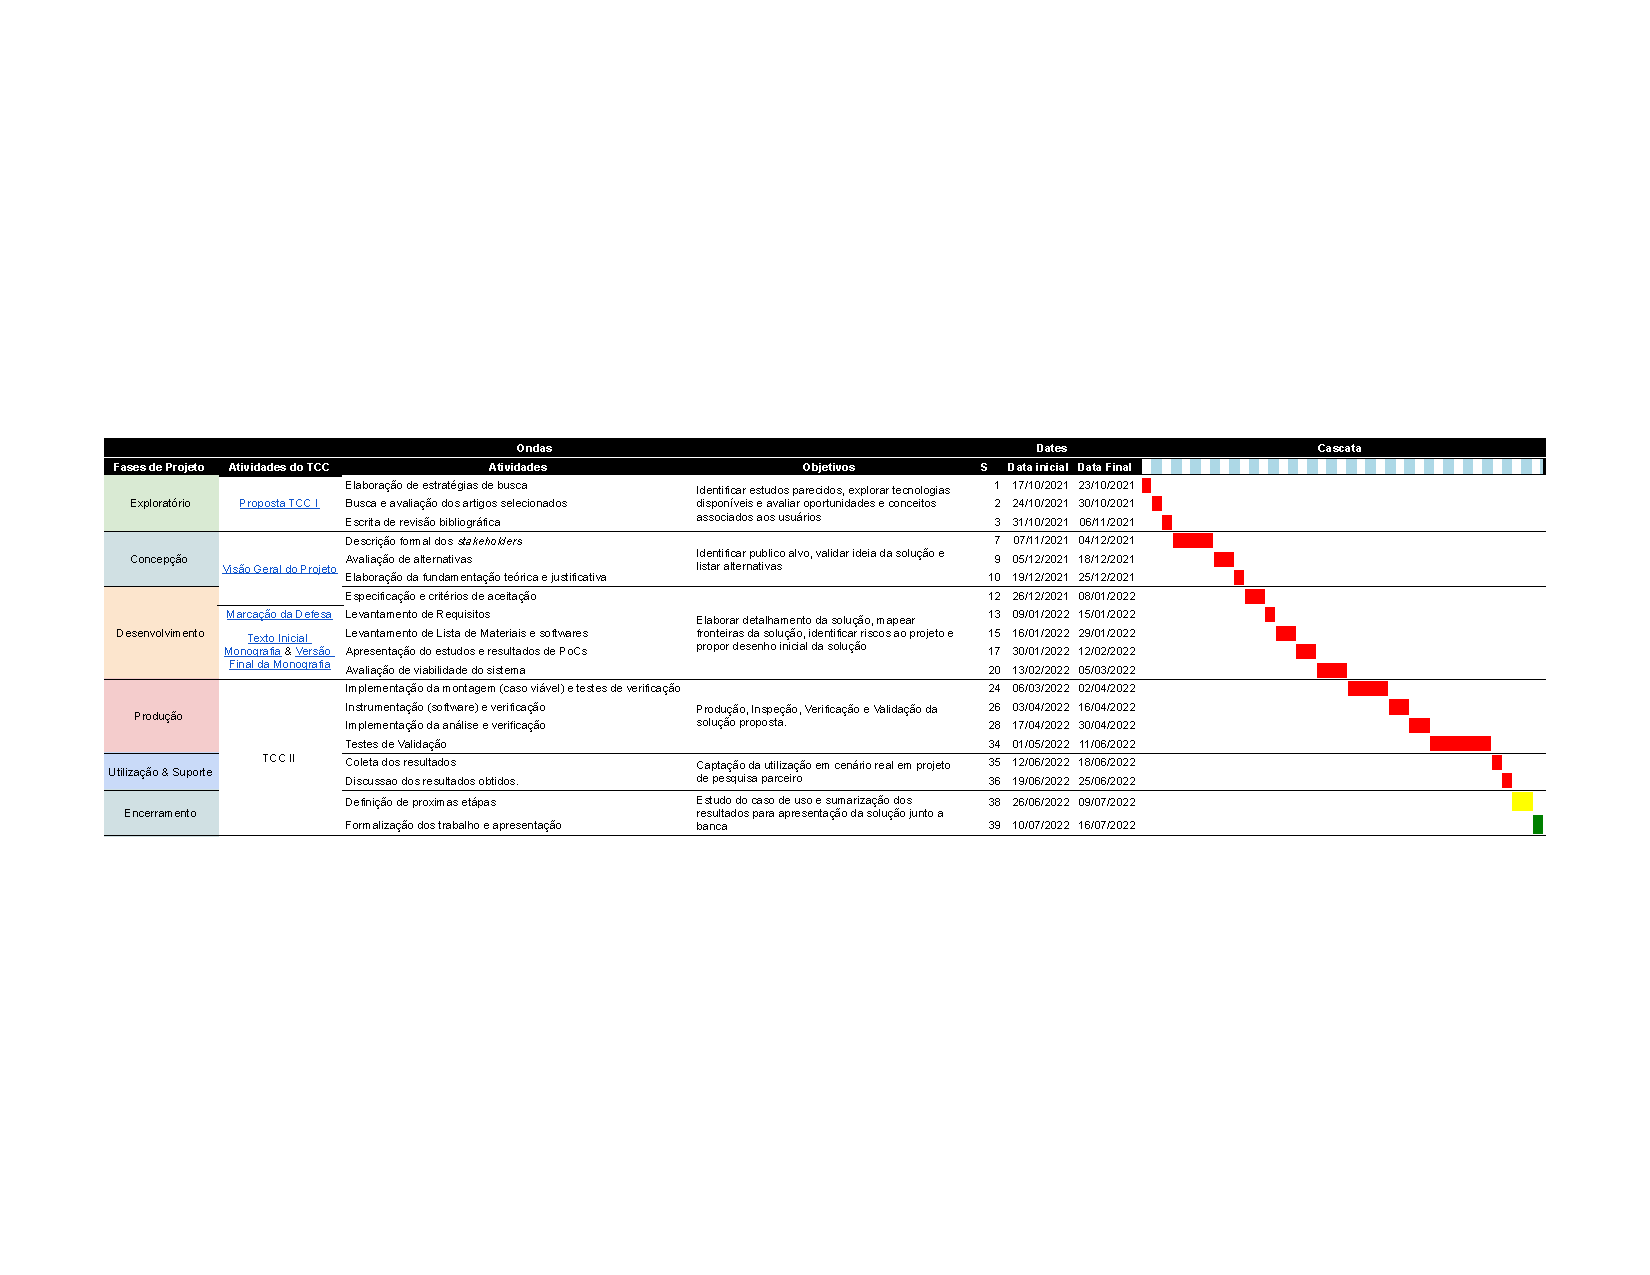
\includegraphics[width=1\linewidth]{04-figuras/TCC cronograma - Sheet1.pdf}
        \caption{Cronograma geral do trabalho}
        \label{fig:cronograma}
    \end{figure}
\end{landscape}